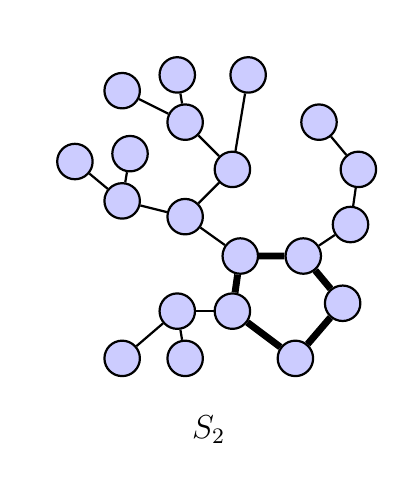
\begin{tikzpicture}[
  baseline=0pt,
  scale=1,
  vnode/.style={circle, draw=black, fill=blue!20, thick, inner sep=0pt, minimum size=4.5mm},
  edge/.style={thick, draw=black},
  bold_edge/.style={line width=2.5pt, draw=black}
]
  \useasboundingbox (-2.3,-3.1) rectangle (2.3,2.4);

  % --- CICLO C^5 (Ubicado en la esquina inferior derecha) ---
  % c3 y c4 son los ÚNICOS dos vértices sin ramas adicionales (grado 2)
  \node[vnode] (c1) at (0.4, -0.5) {};   % Conecta con Rama 1 (Arriba-Izquierda)
  \node[vnode] (c2) at (1.2, -0.5) {};   % Conecta con Rama 2 (Arriba-Derecha)
  \node[vnode] (c3) at (1.7, -1.1) {};   % Vértice limpio (grado 2)
  \node[vnode] (c4) at (1.1, -1.8) {};   % Vértice limpio (grado 2, límite inferior)
  \node[vnode] (c5) at (0.3, -1.2) {};   % Conecta con Rama 3 (Abajo-Izquierda)

  % Aristas del C^5 (reteñidas)
  \draw[bold_edge] (c1) -- (c2) -- (c3) -- (c4) -- (c5) -- (c1);

  % --- RAMA 1: Sale de c5 (3 vértices hacia abajo/izquierda) ---
  \node[vnode] (v6) at (-0.4, -1.2) {};
  \node[vnode] (v7) at (-1.1, -1.8) {};  % Límite inferior
  \node[vnode] (v8) at (-0.3, -1.8) {};  % Límite inferior

  \draw[edge] (c5) -- (v6);
  \draw[edge] (v6) -- (v7);
  \draw[edge] (v6) -- (v8);

  % --- RAMA 2: Sale de c2 (3 vértices hacia la derecha/arriba) ---
  \node[vnode] (v9)  at (1.8, -0.1) {};
  \node[vnode] (v10) at (1.9, 0.6) {};
  \node[vnode] (v11) at (1.4, 1.2) {};

  \draw[edge] (c2) -- (v9);
  \draw[edge] (v9) -- (v10);
  \draw[edge] (v10) -- (v11);

  % --- RAMA 3: Sale de c1 (9 vértices hacia arriba e izquierda) ---
  \node[vnode] (v12) at (-0.3, 0.0) {};
  \node[vnode] (v13) at (-1.1, 0.2) {};
  \node[vnode] (v14) at (-1.7, 0.7) {};
  \node[vnode] (v15) at (-1.0, 0.8) {};
  \node[vnode] (v16) at (0.3, 0.6) {};
  \node[vnode] (v17) at (-0.3, 1.2) {};
  \node[vnode] (v18) at (-1.1, 1.6) {};
  \node[vnode] (v19) at (-0.4, 1.8) {};  % Límite superior
  \node[vnode] (v20) at (0.5, 1.8) {};   % Límite superior

  \draw[edge] (c1) -- (v12);
  \draw[edge] (v12) -- (v13);
  \draw[edge] (v13) -- (v14);
  \draw[edge] (v13) -- (v15);
  \draw[edge] (v12) -- (v16);
  \draw[edge] (v16) -- (v17);
  \draw[edge] (v17) -- (v18);
  \draw[edge] (v17) -- (v19);
  \draw[edge] (v16) -- (v20);

  % Etiqueta
  \node[font=\large] at (0,-2.7) {$S_2$};
\end{tikzpicture}
